Die Grundlage für das Schweben des Luftkissenbootes ist der auf den Boden gerichtete Luftstrom. Die Luft wird vertikal stark nach unten geleitet, wo ein Luftpolster entsteht. 
Durch ein Loch im Boden des Hovercrafts kann die Luft entweichen und somit einen Druck erzeugen, um das Luftkissenboot zum Schweben zu bringen. \\
Mithilfe von Fahnen, welche hinter dem Propeller am Boot angebracht sind, lässt sich das Hovercraft lenken. \\ Für eine vereinfachte Darstellung der Funktionsweise siehe 
\autoref{fig:Funktionsprinzip}. Die blauen Pfeile stellen den Luftstrom dar, der zuerst senkrecht auf den Boden gerichtet ist und danach während des Schwebezustandes unter dem Boot
entweicht. Die vertikalen blauen Pfeile stellen den Luftstrom dar, der durch den hinteren Propeller und die Fahnen geleitet wird. 

\begin{figure}[H]
  \centering
  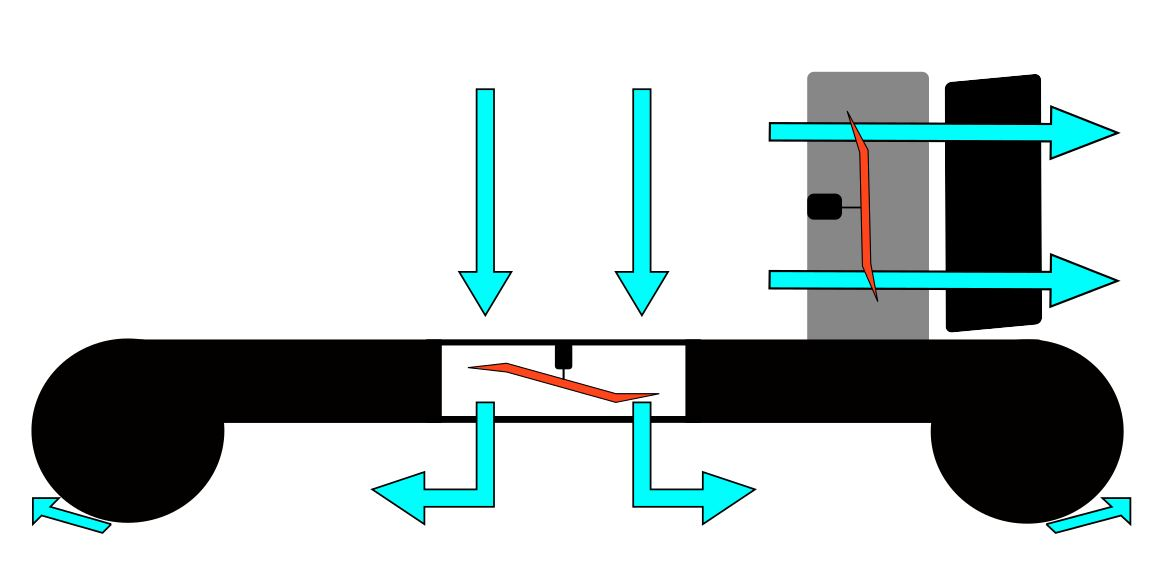
\includegraphics[width=0.9\textwidth]{Fotos/Funktionsprinzip.JPG}
  \caption{Funktionsprinzip eines Hovercrafts  \label{fig:Funktionsprinzip}}
\end{figure}